\section{Диаграммы Эйлера}

Логические операции над множествами допускают простую геометрическую
интерпретацию. В качестве унитарного множества $I$ возьмем плоскость, на
которой будем изображать множества в виде некоторых областей. Тогда
множество $A\cap B$ будет представлять собой область (заштрихованную),
показанную на рис.~1,~\emph{а}. Области (заштрихованные), соответствующие
операциям $A\cup B$, $A\setminus B$, $A\sd B$ и $\ov A$, показаны на рис.~1,
\emph{б}, \emph{в}, \emph{г} и \emph{д} соответственно.

\begin{figure}[h]
\centering
\tikzset{hat/.style={pattern=north east lines,pattern color=black!70}}
\def\ca{(0,0) circle (0.8)}
\def\cb{(0.7,-0.5) circle (0.8)}
\begin{tikzpicture}[scale=0.9]
 \begin{scope}\clip\ca; \fill[hat]\cb; \end{scope}
 \draw\ca node[left=6pt]{$A$}; \draw\cb node[right=4pt]{$B$};
 \node at (0.35,-1.6){\emph{а}}; \node at (0.35,-1.95){\small $A\cap B$};
\end{tikzpicture}\quad
\begin{tikzpicture}[scale=0.9]
 \fill[hat]\ca; \fill[hat]\cb;
 \draw\ca node[left=6pt]{$A$}; \draw\cb node[right=4pt]{$B$};
 \node at (0.35,-1.6){\emph{б}}; \node at (0.35,-1.95){\small $A\cup B$};
\end{tikzpicture}\quad
\begin{tikzpicture}[scale=0.9]
 \begin{scope}[even odd rule]\clip\cb (-2,-2) rectangle (2,2); \fill[hat]\ca; \end{scope}
 \draw\ca node[left=6pt]{$A$}; \draw\cb node[right=4pt]{$B$};
 \node at (0.35,-1.6){\emph{в}}; \node at (0.35,-1.95){\small $A\setminus B$};
\end{tikzpicture}\quad
\begin{tikzpicture}[scale=0.9]
 \fill[hat,even odd rule]\ca \cb;
 \draw\ca node[left=6pt]{$A$}; \draw\cb node[right=4pt]{$B$};
 \node at (0.35,-1.6){\emph{г}}; \node at (0.35,-1.95){\small $A\sd B$};
\end{tikzpicture}\quad
\begin{tikzpicture}[scale=0.9]
 \fill[hat,even odd rule](-1.2,-1.2) rectangle (1.2,1.2) (0,0) circle (0.7);
 \draw (0,0) circle (0.7) node{$A$};
 \node at (0,-1.6){\emph{д}}; \node at (0,-1.95){\small $\ov A$};
\end{tikzpicture}
\figcap{Рис. 1.}
\end{figure}

\begin{figure}[h]
\centering
\begin{tikzpicture}[scale=0.9]
 \def\a{(0,0) circle (0.9)}\def\b{(1.2,0) circle (0.9)}\def\c{(0.6,-1.0) circle (0.9)}
 \fill[pattern=north east lines,pattern color=black!70,even odd rule]\a\b\c;
 \begin{scope}\clip\a;\clip\b;\fill[pattern=north east lines,pattern color=black!70]\c;\end{scope}
 \draw\a node[left=6pt]{$A$};\draw\b node[right=6pt]{$B$};\draw\c node[below=6pt]{$C$};
\end{tikzpicture}
\figcap{Рис. 2.}
\end{figure}

\bookpage{18}%
Применение этих диаграмм, названных диаграммами Эйлера, во многих случаях
позволяет существенно упростить решение задач.

Рассмотрим, например, упражнение~2 \S\,1. Формальное доказательство
ассоциативности симметрической разности $A\sd B$ потребовало выполнения ряда
тождественных преобразований. Построим диаграмму Эйлера для выражения
$A\sd(B\sd C)$ (рис.~2). Из диаграммы видно, что область $A\sd(B\sd C)$
симметрична относительно множеств $A$, $B$, $C$, и такую же диаграмму имеет
множество $(A\sd B)\sd C$.

\begin{figure}[h]
\centering
\begin{tikzpicture}[scale=0.85]
 \draw (0,0) circle (0.8); \draw (0.8,-0.6) circle (0.8);
 \node at (-0.45,0.35){$A$}; \node at (-0.25,-0.15){\small 2};
 \node at (0.45,-0.3){\small 1}; \node at (1.05,-0.95){\small 3};
 \node at (1.25,-0.4){$B$}; \node at (1.7,0.7){\small 4};
 \node at (0.4,-1.8){\emph{а}};
\end{tikzpicture}\qquad\qquad
\begin{tikzpicture}[scale=0.85]
 \draw (0,0) circle (0.9) node[left=4pt]{$A$};
 \draw (1.2,0) circle (0.9) node[right=4pt]{$B$};
 \draw (0.6,-1.0) circle (0.9); \node at (0.95,-1.4){$C$};
 \node at (0.6,0.45){\small 2}; \node at (0.6,-0.35){\small 1};
 \node at (0.05,-0.6){\small 4}; \node at (1.15,-0.6){\small 3};
 \node at (0.35,-1.45){\small 6}; \node at (-0.9,-0.9){\small 7};
 \node at (2.1,-0.6){\small 5}; \node at (2.3,-1.4){\small 8};
 \node at (0.6,-2.3){\emph{б}};
\end{tikzpicture}
\figcap{Рис. 3.}
\end{figure}

Заметим, что диаграммами Эйлера удобно пользоваться лишь при небольшом
числе рассматриваемых областей. С увеличением их числа трудность построения
диаграмм быстро возрастает. Дело в том, что граница каждой следующей
области, изображаемой на диаграмме, должна обязательно пересекаться
с каждой из логически возможных подобластей, на которые предыдущие заданные
области разбивают плоскость. (В противном случае некоторые логически
возможные ситуации могут быть пропущены.) Так, одной области $A$
соответствуют две подобласти плоскости $\R^2$: сама область $A$ и ее
внешность $\ov A$. Двум областям $A$ и $B$ соответствуют уже четыре
подобласти (рис.~3,~\emph{а}), а трем подобластям "--- восемь
(рис.~3,~\emph{б}). Такие области будем называть \emph{конституентными
областями}. Очевидно, подобрать четвертую область $D$, граница которой
проходила бы через внутренние точки каждой из подобластей, уже труднее
(рис.~4). Заметим, что если, например, вместо рис.~3,~\emph{б} принять
расположение областей такое, как показано на рис.~5, то логической формуле
$(A\cap B)\cap C$ соответствовало бы пустое множество $\emptyset$, что для
других множеств $A$, $B$ и $C$, вообще, не верно.

\begin{figure}[h]
\centering
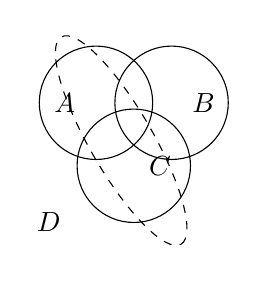
\begin{tikzpicture}[scale=0.8]
 \draw (0,0) circle (0.9) node[left=4pt]{$A$};
 \draw (1.2,0) circle (0.9) node[right=4pt]{$B$};
 \draw (0.6,-1.0) circle (0.9) node[right=2pt]{$C$};
 \draw[dashed,rotate around={-60:(0.4,-0.6)}] (0.4,-0.6) ellipse (1.9 and 0.5);
 \node at (-0.75,-1.9){$D$};
\end{tikzpicture}
\figcap{Рис. 4.}
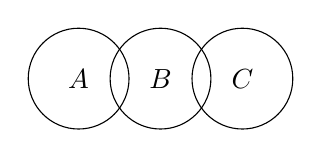
\begin{tikzpicture}[scale=0.8]
 \draw (0,0) circle (0.8) node{$A$};
 \draw (1.3,0) circle (0.8) node{$B$};
 \draw (2.6,0) circle (0.8) node{$C$};
\end{tikzpicture}
\figcap{Рис. 5.}
\end{figure}

\subsection*{Упражнения и задачи}
1. Используя диаграммы Эйлера, доказать тождества\fixed{в оригинале последнее тождество напечатано как
$A\cup[(B\setminus\ov A)\sd C]\equiv(A\cap B)\sd C$, которое тождеством
не является (при $A=I$, $B=C=\emptyset$ левая часть равна $I$, правая "---
$\emptyset$). Восстановленный вариант и разбор "--- в решении ниже.}
\[
\begin{gathered}
(A\cup C)\cap B\equiv(A\cap B)\cup(\ov A\cap B\cap C);\\
[A\cap(B\cup C)]\cup(\ov A\cap C)\equiv C\cup(A\cap B);\\
(A\cap C)\cup(B\cap C)\cup(C\setminus A)\equiv C;\qquad A\sd B\equiv(A\cup B)\setminus(A\cap B);\\
[A\cap(B\sd C)]\cup(B\sd C)\equiv B\sd C;\\
A\cap[(B\setminus\ov A)\sd C]\equiv(A\cap B)\sd(A\cap C).
\end{gathered}
\]


\bookpage{19}%
2. Выпуклые области $A,B,C\subset\R^2$ разбивают плоскость на восемь частей,
различающихся состояниями принадлежности их точек множествам $A$, $B$ и $C$.
Может ли добавление выпуклой области $D$ привести к разбиению $\R^2$ на 16
подобластей указанного типа? Какое максимальное число таких подобластей
могут образовать $n$ выпуклых областей в $\R^2$?

3. Существуют ли (для всякого $n$) конгруэнтные (т.\,е. получающиеся одна из
другой переносом и поворотом) области $A_1,\dots,A_n\subset\R^2$,
разбивающие плоскость на максимально возможное ($2^n$) число частей, которые
различаются между собой состояниями принадлежности их точек областям
$A_1,\dots,A_n$. (Заметим, что для $n\le3$ такими областями, например,
являются круги одинакового радиуса.)

%======================================================================
\begin{solution}[1 (\S\,2)]
Нумеруем конституентные области трех кругов, как на рис.~3,~\emph{б},
и записываем, какие из них образуют левую и правую части. Удобнее
обозначать область тройкой $\alpha\beta\gamma$ состояний принадлежности
к $A$, $B$, $C$ ($1$ "--- внутри, $0$ "--- вне); тогда
\[
1=111,\ 2=110,\ 3=011,\ 4=101,\ 5=010,\ 6=001,\ 7=100,\ 8=000 .
\]
\begin{center}\small
\begin{tabular}{lll}
\toprule
тождество & левая часть & правая часть\\
\midrule
$(A\cup C)\cap B\equiv(A\cap B)\cup(\ov A\cap B\cap C)$ & $\{1,2,3\}$ & $\{1,2\}\cup\{3\}$\\
$[A\cap(B\cup C)]\cup(\ov A\cap C)\equiv C\cup(A\cap B)$ & $\{1,2,4\}\cup\{3,6\}$ & $\{1,3,4,6\}\cup\{1,2\}$\\
$(A\cap C)\cup(B\cap C)\cup(C\setminus A)\equiv C$ & $\{1,4\}\cup\{1,3\}\cup\{3,6\}$ & $\{1,3,4,6\}$\\
$A\sd B\equiv(A\cup B)\setminus(A\cap B)$ & $\{4,7,3,5\}$ & $\{1,\dots,5,7\}\setminus\{1,2\}$\\
$[A\cap(B\sd C)]\cup(B\sd C)\equiv B\sd C$ & $\{2,4\}\cup\{2,4,5,6\}$ & $\{2,4,5,6\}$\\
\bottomrule
\end{tabular}
\end{center}
Во всех строках множества номеров совпадают, а так как три круга
в положении рис.~3,~\emph{б} реализуют все восемь логически возможных
состояний, совпадение областей на диаграмме и означает тождество
(см. также упр.~2 \S\,3 и решение упр.~7 \S\,3, где это рассуждение
обосновано строго). Четвертое и пятое тождества видны уже на диаграмме
двух кругов (пятое "--- это поглощение $(X\cap Y)\cup Y\equiv Y$).

\emph{Последнее тождество.} Поскольку $B\setminus\ov A\equiv B\cap A$,
напечатанное в книге равенство
$A\cup[(B\setminus\ov A)\sd C]\equiv(A\cap B)\sd C$ имеет левую часть
$A\cup\{1,2\}\sd\{1,3,4,6\}=\{1,2,4,7\}\cup\{2,3,4,6\}=\{1,2,3,4,6,7\}$,
а правую $\{2,3,4,6\}$: они различаются областями $1$ и $7$ (например, при
$A=I$, $B=C=\emptyset$). Значит, в книге опечатка. Естественный
верный вариант "--- с пересечением вместо объединения:
\[
A\cap[(B\setminus\ov A)\sd C]\equiv(A\cap B)\sd(A\cap C):
\]
слева $\{1,2,4,7\}\cap\{2,3,4,6\}=\{2,4\}$, справа
$\{1,2\}\sd\{1,4\}=\{2,4\}$. Это тождество выражает
дистрибутивность $\cap$ относительно $\sd$:
$A\cap(X\sd Y)\equiv(A\cap X)\sd(A\cap Y)$. (Верно также
$A\cap[(B\setminus\ov A)\sd C]\equiv(A\cap B)\sd(A\cap C)\equiv A\cap(B\sd C)$.)
\end{solution}

\begin{solution}[2 (\S\,2)]
\emph{Ответ: да; $n$ выпуклых областей могут дать все $2^n$
логически возможных частей.}

Для $n=4$ это показывает, например, известная диаграмма Венна из четырех
равных эллипсов (эллипс выпуклый). Общая конструкция для любого $n$:
возьмем на окружности $2^n$ различных точек $q_\alpha$, занумерованных
наборами $\alpha=(\alpha_1,\dots,\alpha_n)\in\{0,1\}^n$, и положим
\[
A_i=\operatorname{conv}\{q_\alpha:\ \alpha_i=1\}
\]
(выпуклая оболочка; чтобы получить область с внутренними точками, ее можно
слегка <<раздуть>>, взяв $\varepsilon$-окрестность при малом
$\varepsilon$ "--- выпуклость сохраняется). Точки на окружности находятся
в выпуклом положении: ни одна из них не лежит в выпуклой оболочке
остальных и даже отстоит от нее на положительное расстояние. Поэтому
$q_\alpha\in A_i\iff\alpha_i=1$, т.\,е. точка $q_\alpha$ принадлежит
конституенте $A_1^{\alpha_1}\cap\dots\cap A_n^{\alpha_n}$, и все $2^n$
конституент непусты (а вместе с малыми окрестностями точек $q_\alpha$,
лежащими вне всех $A_i$ с $\alpha_i=0$, "--- имеют внутренние точки).

Итак, максимальное число частей, различающихся состояниями
принадлежности, равно $2^n$ "--- больше быть не может, так как наборов
состояний всего $2^n$. (Связными эти части, вообще говоря, не будут; если
же считать связные компоненты, то их число для выпуклых областей не
ограничено никакой функцией от $n$: границы двух выпуклых многоугольников
могут пересекаться в сколь угодно большом числе точек.)
\end{solution}

\begin{solution}[3 (\S\,2)]
\emph{Ответ: да, для всякого $n$; можно даже обойтись одними
параллельными переносами.}

Выберем $n$ векторов $v_1,\dots,v_n$ и $2^n$ точек $x_\alpha$,
$\alpha\in\{0,1\}^n$, <<в общем положении>>, так чтобы все $n2^n$ точек
$x_\alpha-v_i$ были попарно различны (этого можно добиться сколь угодно
малым шевелением). Разобьем их на два конечных множества
\[
P_+=\{x_\alpha-v_i:\ \alpha_i=1\},\qquad P_-=\{x_\alpha-v_i:\ \alpha_i=0\}.
\]
Пусть $S$ "--- связная открытая область, содержащая все точки $P_+$ и не
содержащая ни одной точки $P_-$ (например, объединение малых кругов вокруг
точек $P_+$, соединенных тонкими <<коридорами>>, обходящими конечное
множество $P_-$, "--- плоскость без конечного множества точек связна).
Положим $A_i=S+v_i$. Тогда
\[
x_\alpha\in A_i\iff x_\alpha-v_i\in S\iff\alpha_i=1,
\]
т.\,е. $x_\alpha$ лежит в конституенте с номером $\alpha$, и все $2^n$
конституент непусты (и открыты в окрестности $x_\alpha$, если круги
выбрать малыми). Области $A_i$ конгруэнтны "--- они получаются друг из
друга переносом.

Для $n\le3$ подходят равные круги (рис.~3,~\emph{б}). Для $n\ge4$
равные (и вообще любые) \emph{круги} уже не годятся: $n$ окружностей
разбивают плоскость не более чем на $n^2-n+2$ связных частей (каждая новая,
$k$-я, окружность пересекает прежние не более чем в $2(k-1)$ точках
и добавляет не более $2(k-1)$ частей). Каждая непустая конституента
содержит хотя бы одну такую часть, поэтому непустых конституент не больше
$n^2-n+2$, а $n^2-n+2<2^n$ при $n\ge4$. Поэтому при $n\ge4$ приходится
брать области более сложной формы, как в построении выше. Для простых $n$
существуют даже симметричные диаграммы Венна из $n$ конгруэнтных кривых,
переходящих друг в друга поворотом (Григгс, Киллиан, Сэвидж, 2004).
\end{solution}
